L’évaluation des performances se décomposent des différents éléments suivants, et qui sont présentés dans le diagramme de la figure \ref{fig:metho_eval}: 
\begin{itemize}
    \item Tout d'abord, les indicateurs de performances.
    \begin{itemize}
        \item Les performances matérielles durant l'inférence sont évaluées grâce aux indicateurs fournies par les utilitaires 'Tegrastats' de NVIDIA, 'free' et 'iotop'. Ces utilitaires sont brièvement décrits dans le tableau \ref{table:table_sol_logiciel}.
        \item Les performances de la segmentation sont évaluées avec les indicateurs classiques\footnote{\url{https://ilmonteux.github.io/2019/05/10/segmentation-metrics.html}}: le "\acrshort{iou}" ("\acrlong{iou}", ou "Jaccard index"); et le F1 score (ou "Dice coefficient").
    \end{itemize}
    \item Ensuite, différentes résolutions d'images et de vidéos sont utilisées pour déterminer lesquelles sont supportées par l'architecture évalué, tel qu'indiqué dans la section "\ref{section:resolutions_to_be_tested} \nameref{section:resolutions_to_be_tested}". 
    \item Les images et vidéos qui sont à notre disposition pour être évaluée proviennent de différentes sources de données, tel que décrit dans la section "\ref{section:collecte_donnees} \nameref{section:collecte_donnees}". 
    \item Enfin plusieurs modèles ont été sélectionnés comme candidats intéressants pour l'évaluation, et décrit dans la section "\ref{section:choix_modele_architecture} \nameref{section:choix_modele_architecture}".
\end{itemize} 
\label{metho_eval}
\begin{figure}[H]
    \centering
    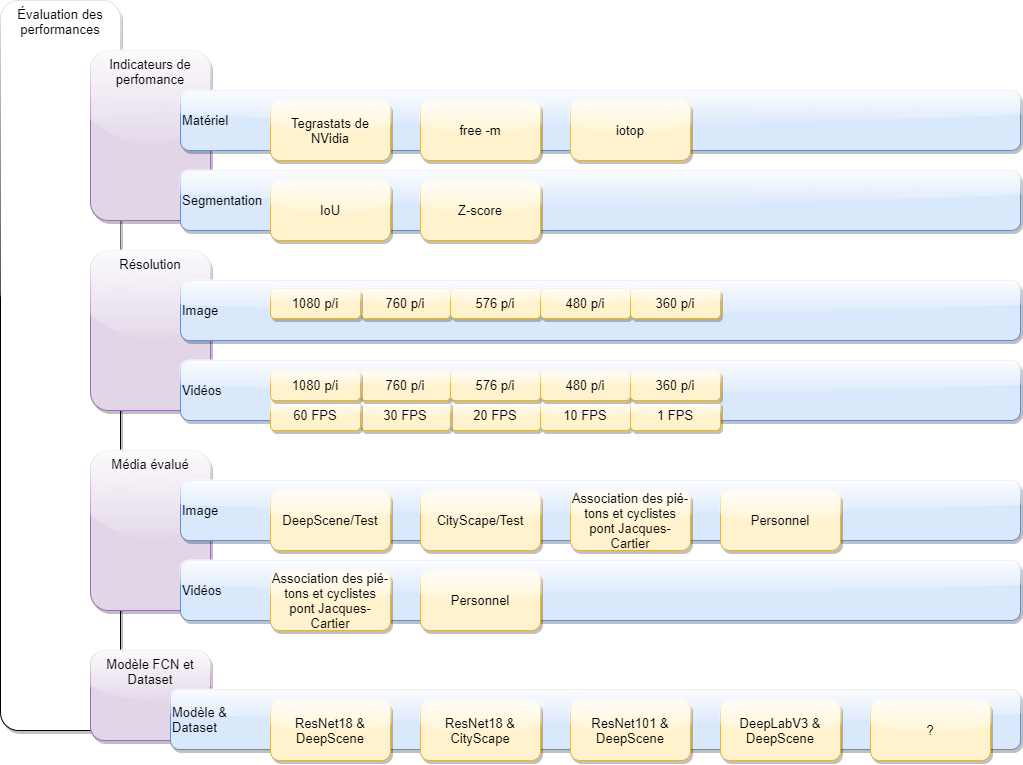
\includegraphics[width=1.0\textwidth]{metho_eval_perf_round_glass_shadow2}
    \caption{Éléments pour l'évaluation des performances}
    \label{fig:metho_eval}
\end{figure}
\subsubsection{Stratégie de test de l'inférence} \label{section:strategie_test_inference}
\noindent L'objectif principal de l'essai est de déterminer la capacité et les limites du nano-ordinateur d'inférer en temps réel des architectures de réseau de neurones pleinement connectés (\acrshort{fcnn}) pour la segmentation sémantique de vidéos. La stratégie qui est appliquée est de tester avec diverses architectures et divers niveaux de qualité vidéos, en espérant trouver le compromis qui répond le mieux à cet objectif.
\begin{enumerate}
   \item \label{metho:testbaseinférence} Afin de s'assurer du bon fonctionnement du nano-ordinateur et d'avoir des résultats de référence propre à notre environnement, l'inférence est testée avec des modèles existants et préentrainés pour la segmentation sémantique, avec les images et les vidéos provenant des références, et dont les caractéristiques et les résultats sont disponibles. 
   \item \label{metho:testbaseinférencesite} En espérant que les tests de l'étape \#\ref{metho:testbaseinférence} donnent les résultats documentés dans les articles de références, ils sont repris avec les mêmes modèles, mais avec les images et les vidéos du site d'étude possédant la meilleure qualité acquise (1080p/i, 30\acrshort{fps}). Les données sources (images et vidéos) devront subir certains pré traitements à ce effet, afin de répondre aux requis des architectures.
   \item \label{metho:testdevinférencesite} Selon les résultats de l'étape \#\ref{metho:testbaseinférencesite}, les tests se concentreront sur l'inférence avec des vidéos, en réduisant progressivement la résolution (760p/i, 576p/i, 480p/i, 360p/i) et le nombre d'images par seconde (20\acrshort{fps}, 10FSP, 1\acrshort{fps}).
   \item Les étapes intermédiaires de l'étape \#\ref{metho:testdevinférencesite} sont de 1) valider les résultats de l'inférence avec des images avant de tester avec les vidéos, et 2) évaluer si les architectures de réseaux de neurones pleinement connectés (\acrshort{fcnn}) doivent et/ou peuvent être adaptées facilement, en tenant compte de l'échéancier de l'essai, et ce afin de répondre à l'objectif principal.
\end{enumerate}
\subsubsection{Stratégie de collecte des indicateurs de performance matériel}
\noindent La méthodologie de la collecte des indicateurs est la suivante\footnote{\url{https://vince7lf.github.io/2020/05/26/metrics.html}}: 
\begin{itemize}
    \item La collecte est démarrée après un démarrage frais, manuellement, via un script shell, qui exécute chaque utilitaire, et attend l'interruption du test.
    \item Chaque utilitaire qui est utilisé pour collecter les mesures, possède son propre fichier.
    \item La date et l'heure de chaque indicateur collecté sont précisées.
    \item Afin de faciliter la documentation et l'analyse du test, des points d'intérêt sont ajoutés dans un fichier séparé pour marquer un moment particulier du test, avec la date, l'heure et un libellé. Ce point d'intérêt est fait grâce à une commande "shell" qui vient ajouter une trace dans ce fichier.
    \item Chaque indicateur est collecté toutes les secondes.
    \item Une fois le test complété, la collecte est arrêtée manuellement. 
    \item Chaque fichier est ensuite transformé en fichier \acrshort{csv}, via des commandes shell.
    \item À partir des fichiers \acrshort{csv} un script Python génère les graphiques automatiquement. 
\end{itemize}
\vspace{0.5\baselineskip}
\noindent Chaque indicateur est une colonne du fichier \acrshort{csv}. Il existe le même nombre d'indicateurs à tout moment. La date et l'heure sont un champ. 
\vspace{0.5\baselineskip}
\\
\noindent Avant tout début de tests, la collecte est démarrée sans activité autre que la collecte des indicateurs. Cela permet de prendre une base de référence sans aucune charge.
\vspace{0.5\baselineskip}
\\
\noindent Ensuite les tests débutent. 
\vspace{0.5\baselineskip}
\\
\noindent Les indicateurs collectés permettent de créer des graphiques qui montrent la progression de chacun.
\vspace{0.5\baselineskip}
\\
\noindent Les performances matérielles du Jetson Nano sont évaluées grâce à différents utilitaires : "tegrastats" fournis par NVIDIA; "free"; et "iotop".
\vspace{0.5\baselineskip}
\\
\noindent Les performances de la segmentation sont évaluées grâce au \acrshort{iou} et au F1 score pour la classe du chemin / route. Une fonction Python est utilisée. Les fonctions \acrshort{iou} et le F1 score utilisent l'image prédite (généré par l'architecture \acrshort{fcn}) et l'image vérité terrain (\acrshort{gt}). Les images originales sont pré sélectionnées selon leur intérêt et l'image vérité terrain (\acrshort{gt}) créée. L'image prédite et vérité terrain (\acrshort{gt}) doivent utiliser la même palette de couleurs et doivent être de la même résolution. Pour les images qui ne possèdent pas d'image vérité terrain (\acrshort{gt}), celle-ci est créée à la main avec l'éditeur "Gimp", en utilisant la même résolution de la segmentation de l'image produite par l'architecture du modèle de NVIDIA. Le besoin est d'évaluer et non d'entrainer, l'importance de la précision de la classification est moindre dans ce cas. 
\subsubsection{Résolutions évaluées}\label{section:resolutions_to_be_tested}
Les résolutions et images par seconde qui sont évaluées sont présentées dans le tableau \ref{table:resolutions_to_be_tested}.
{
    \renewcommand*{\arraystretch}{1.4}
    \begin{table}[ht]
    \centering
    \caption{Résolutions et images par seconde (\acrshort{fps}) qui sont évaluées}\label{table:resolutions_to_be_tested}
    \vspace{0.1em} % Adjust the height of the space between caption and tabular
    \begin{tabular}{{@{}|p{35em}|@{}}}
         \hline
         \textbf{Résolutions}\\
         \hline
        320x576, 480x640, 720x1280, 768x1024, 768x1152, 800x1152, 832x1024, 864x1024, 832x1120, 832x1152, 768x1280, 800x1280, 864x1152, 900x1152, 900x1280, 960x1600, 1080x1920, 1024x1024\\
        \hline
        \textbf{Images par seconde (\acrshort{fps}) }\\
        \hline
        60/1, 30/1, 15/1, 1/1\\
        \hline
    \end{tabular}
    \end{table}
}